\documentclass[11pt,preprint, authoryear]{elsarticle}

\usepackage{lmodern}
%%%% My spacing
\usepackage{setspace}
\setstretch{1.2}
\DeclareMathSizes{12}{14}{10}{10}

% Wrap around which gives all figures included the [H] command, or places it "here". This can be tedious to code in Rmarkdown.
\usepackage{float}
\let\origfigure\figure
\let\endorigfigure\endfigure
\renewenvironment{figure}[1][2] {
    \expandafter\origfigure\expandafter[H]
} {
    \endorigfigure
}

\let\origtable\table
\let\endorigtable\endtable
\renewenvironment{table}[1][2] {
    \expandafter\origtable\expandafter[H]
} {
    \endorigtable
}


\usepackage{ifxetex,ifluatex}
\usepackage{fixltx2e} % provides \textsubscript
\ifnum 0\ifxetex 1\fi\ifluatex 1\fi=0 % if pdftex
  \usepackage[T1]{fontenc}
  \usepackage[utf8]{inputenc}
\else % if luatex or xelatex
  \ifxetex
    \usepackage{mathspec}
    \usepackage{xltxtra,xunicode}
  \else
    \usepackage{fontspec}
  \fi
  \defaultfontfeatures{Mapping=tex-text,Scale=MatchLowercase}
  \newcommand{\euro}{€}
\fi

\usepackage{amssymb, amsmath, amsthm, amsfonts}

\def\bibsection{\section*{References}} %%% Make "References" appear before bibliography


\usepackage[round]{natbib}

\usepackage{longtable}
\usepackage[margin=2.3cm,bottom=2cm,top=2.5cm, includefoot]{geometry}
\usepackage{fancyhdr}
\usepackage[bottom, hang, flushmargin]{footmisc}
\usepackage{graphicx}
\numberwithin{equation}{section}
\numberwithin{figure}{section}
\numberwithin{table}{section}
\setlength{\parindent}{0cm}
\setlength{\parskip}{1.3ex plus 0.5ex minus 0.3ex}
\usepackage{textcomp}
\renewcommand{\headrulewidth}{0.2pt}
\renewcommand{\footrulewidth}{0.3pt}

\usepackage{array}
\newcolumntype{x}[1]{>{\centering\arraybackslash\hspace{0pt}}p{#1}}

%%%%  Remove the "preprint submitted to" part. Don't worry about this either, it just looks better without it:
\makeatletter
\def\ps@pprintTitle{%
  \let\@oddhead\@empty
  \let\@evenhead\@empty
  \let\@oddfoot\@empty
  \let\@evenfoot\@oddfoot
}
\makeatother

 \def\tightlist{} % This allows for subbullets!

\usepackage{hyperref}
\hypersetup{breaklinks=true,
            bookmarks=true,
            colorlinks=true,
            citecolor=blue,
            urlcolor=blue,
            linkcolor=blue,
            pdfborder={0 0 0}}


% The following packages allow huxtable to work:
\usepackage{siunitx}
\usepackage{multirow}
\usepackage{hhline}
\usepackage{calc}
\usepackage{tabularx}
\usepackage{booktabs}
\usepackage{caption}


\newenvironment{columns}[1][]{}{}

\newenvironment{column}[1]{\begin{minipage}{#1}\ignorespaces}{%
\end{minipage}
\ifhmode\unskip\fi
\aftergroup\useignorespacesandallpars}

\def\useignorespacesandallpars#1\ignorespaces\fi{%
#1\fi\ignorespacesandallpars}

\makeatletter
\def\ignorespacesandallpars{%
  \@ifnextchar\par
    {\expandafter\ignorespacesandallpars\@gobble}%
    {}%
}
\makeatother

\newlength{\cslhangindent}
\setlength{\cslhangindent}{1.5em}
\newenvironment{CSLReferences}%
  {\setlength{\parindent}{0pt}%
  \everypar{\setlength{\hangindent}{\cslhangindent}}\ignorespaces}%
  {\par}


\urlstyle{same}  % don't use monospace font for urls
\setlength{\parindent}{0pt}
\setlength{\parskip}{6pt plus 2pt minus 1pt}
\setlength{\emergencystretch}{3em}  % prevent overfull lines
\setcounter{secnumdepth}{5}

%%% Use protect on footnotes to avoid problems with footnotes in titles
\let\rmarkdownfootnote\footnote%
\def\footnote{\protect\rmarkdownfootnote}
\IfFileExists{upquote.sty}{\usepackage{upquote}}{}

%%% Include extra packages specified by user

%%% Hard setting column skips for reports - this ensures greater consistency and control over the length settings in the document.
%% page layout
%% paragraphs
\setlength{\baselineskip}{12pt plus 0pt minus 0pt}
\setlength{\parskip}{12pt plus 0pt minus 0pt}
\setlength{\parindent}{0pt plus 0pt minus 0pt}
%% floats
\setlength{\floatsep}{12pt plus 0 pt minus 0pt}
\setlength{\textfloatsep}{20pt plus 0pt minus 0pt}
\setlength{\intextsep}{14pt plus 0pt minus 0pt}
\setlength{\dbltextfloatsep}{20pt plus 0pt minus 0pt}
\setlength{\dblfloatsep}{14pt plus 0pt minus 0pt}
%% maths
\setlength{\abovedisplayskip}{12pt plus 0pt minus 0pt}
\setlength{\belowdisplayskip}{12pt plus 0pt minus 0pt}
%% lists
\setlength{\topsep}{10pt plus 0pt minus 0pt}
\setlength{\partopsep}{3pt plus 0pt minus 0pt}
\setlength{\itemsep}{5pt plus 0pt minus 0pt}
\setlength{\labelsep}{8mm plus 0mm minus 0mm}
\setlength{\parsep}{\the\parskip}
\setlength{\listparindent}{\the\parindent}
%% verbatim
\setlength{\fboxsep}{5pt plus 0pt minus 0pt}



\begin{document}



\begin{frontmatter}  %

\title{App data from Google Play Store}

% Set to FALSE if wanting to remove title (for submission)




\author[Add1]{Ruan Geldenhuys}
\ead{\href{mailto:22550801@sun.ac.za}{\nolinkurl{22550801@sun.ac.za}}}





\address[Add1]{Stellenbosch University, Stellenbosch, South Africa}


\begin{abstract}
\small{
This document investigates what makes applications on the Google Play
Store successful by using publicaly available data regarding app
information. By comparing app level characteristics, it is possible to
gain insight into why some apps outperform others.
}
\end{abstract}

\vspace{1cm}





\vspace{0.5cm}

\end{frontmatter}



%________________________
% Header and Footers
%%%%%%%%%%%%%%%%%%%%%%%%%%%%%%%%%
\pagestyle{fancy}
\chead{}
\rhead{}
\lfoot{}
\rfoot{}
\lhead{}
%\rfoot{\footnotesize Page \thepage } % "e.g. Page 2"
\cfoot{}

%\setlength\headheight{30pt}
%%%%%%%%%%%%%%%%%%%%%%%%%%%%%%%%%
%________________________

\headsep 35pt % So that header does not go over title




\hypertarget{price-range-and-downloads}{%
\subsection{Price Range and Downloads}\label{price-range-and-downloads}}

Below is a table that displays different price ranges for apps, together
with the median and average downloads for that price range. The table is
sorted by average downloads.

\begin{table}[ht]
\centering
\begin{tabular}{rlrr}
  \hline
 & Price Range & Median Downloads & Average Downloads \\ 
  \hline
1 & 0 & 100000.00 & 9386441.29 \\ 
  2 & 5-10 & 1000.00 & 180813.16 \\ 
  3 & 0-5 & 1000.00 & 70708.07 \\ 
  4 & 20-25 & 10000.00 & 24040.00 \\ 
  5 & 10-15 & 5000.00 & 19598.33 \\ 
  6 & 40+ & 1000.00 & 8884.84 \\ 
  7 & 25-30 & 1000.00 & 6003.44 \\ 
  8 & 15-20 & 1000.00 & 5507.50 \\ 
  9 & 30-35 & 1000.00 & 666.67 \\ 
  10 & 35-40 & 100.00 & 368.33 \\ 
   \hline
\end{tabular}
\caption{Price vs Downloads} 
\end{table}

It is clear from the table that cheaper apps garner more downloads.
While this correlation is not perfect it does roughly hold across the
different price ranges. This effect is to expected in any product, not
just apps. When building an app it is important to consider the
trade-off between the upfront revenue versus ad-revenue. This data shows
that it is a possibility that ad-revenue could outperform upfront
revenue since the difference in downloads between price ranges is so
large.

Note however, these average could be blown out of proportion due to
hyper-successful outliers. The counter argument to that however, is the
fact that for every successful app, there is likely to be an app that
gets almost no downloads.

\hypertarget{categories-of-apps}{%
\subsection{Categories of Apps}\label{categories-of-apps}}

The graph below shows the top ten categories of apps on the Google Play
Store. The bars indicate average downloads, while the line represents
the average size of the apps in the category.
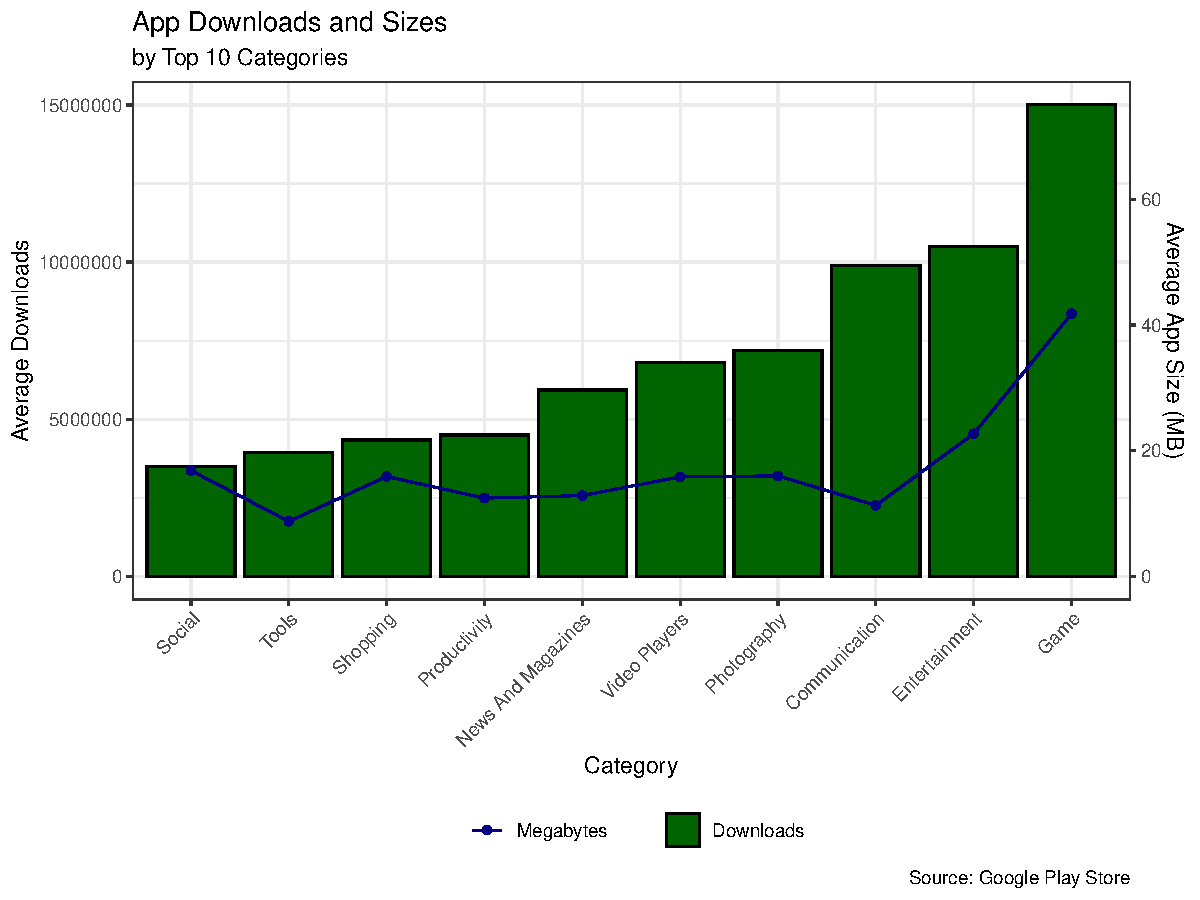
\includegraphics{Question5_files/figure-latex/unnamed-chunk-3-1.pdf}

Gaming apps are by far the most popular app on the Google Play Store,
followed by Entertainment and Communication. When comparing the relative
popularity of apps to their sizes, one might be tempted to infer that
larger apps perform better. However, this relationship only holds for
the top three categories, and is therefore likely not causal. Most apps,
apart from gaming, fall around the 20 MB range. Thus, when developing an
app we should aim for this size, as much larger might deter users since
modern phones don't accommodate external storage.

Furthermore, one should be wary of simply building a mobile app because
gaming is the most popular category, since this market is likely to be
saturated. Instead more market research is needed before committing to a
single category of app.

-Ruan Geldenhuys

\bibliography{Tex/ref}





\end{document}
